\documentclass[14pt, a4paper]{article}
\usepackage[utf8]{inputenc}
\usepackage[russian]{babel}
\usepackage{multirow}
\usepackage{graphicx}

\title{\textbf{Отчет о выполнении лабораторной работы 1.4.2}}
\author{Калашников Михаил, Б03-205}
\date{}

\begin{document}

\maketitle

\textbf{Цель работы:} исследовать вынужденную прецессию гироскопа; установить зависимость скорости вынужденной прецессии от величины момента сил, действующих на ось гироскопа; определить скорость вращения ротора гироскопа и сравнить ее со скоростью, рассчитанной по скорости прецессии.
\newline
\par
Измерим период вынужденной прецессии гироскопа с помощью пяти грузиков различной массы. Нагружая гироскоп, измерим время, за которое ось гироскопа совершит целое количество оборотов и занесем в таблицу. Рассчитаем средний период обращения для каждого значения массы.

\begin{table}[!h]
\centering
\begin{tabular}{| c | c | c | c | c | c | c | c | c | c |}
\hline
\multicolumn{2}{| c |}{$m=335\ g$} & \multicolumn{2}{| c |}{$m=273\ g$} & \multicolumn{2}{| c |}{$m=220\ g$} & \multicolumn{2}{| c |}{$m=176\ g$} & \multicolumn{2}{| c |}{$m=141\ g$} \\
\hline
$N$ & $t$, $min$ & $N$ & $t$, $min$ & $N$ & $t$, $min$ & $N$ & $t$, $min$ & $N$ & $t$, $min$ \\
\hline
7 & 03:36.26 & 4 & 02:32.40 & 2 & 01:39.03 & 2 & 01:57.51 & 2 & 02:24.89 \\
3 & 01:33.80 & 2 & 01:14.80 & 2 & 01:39.05 & 2 & 01:57.40 & 2 & 02:26.50 \\
3 & 01:32.83 & 3 & 01:54.60 & 2 & 01:39.54 & 2 & 01:58.87 & 2 & 02:25.44 \\
4 & 02:03.49 & 3 & 01:54.90 & 2 & 01:39.46 & 2 & 01:59.25 & 2 & 02:26.96 \\
6 & 03:05.77 & 3 & 01:55.44 & 2 & 01:34.55 & 2 & 01:57.88 & 2 & 02:24.88 \\
\hline
\multicolumn{2}{| c |}{$T=31\pm 0.1\ s$} & \multicolumn{2}{| c |}{$T=38\pm 0.2\ s$} & \multicolumn{2}{| c |}{$T=49\pm 0.5\ s$} & \multicolumn{2}{| c |}{$T=59\pm 0.2\ s$} & \multicolumn{2}{| c |}{$T=73\pm 0.2\ s$} \\
\hline
\end{tabular}
\label{table1}
\caption{Измерения периода вынужденной прецессии гироскопа}
\end{table}

На основе вычисленного периода определим угловую частоту прецессии $\Omega$ и построим график зависимости данной частоты от массы нагрузки гироскопа $m$. С помощью МНК определим коэффициент наклона прямой $k$.

\[\Omega=\frac{2\pi}{T}\]
\[\sigma_{\Omega}=\Omega\frac{\sigma_T}{T}\]

\begin{table}[!h]
\centering
\begin{tabular}{| c | c | c |}
\hline
N & $m$, $g$ & $\Omega$, $10^3\ s^{-1}$ \\
\hline
1 & 335 & $203\pm 0.5$ \\
2 & 273 & $165\pm 0.8$ \\
3 & 220 & $128\pm 1.2$ \\
4 & 176 & $106\pm 0.3$ \\
5 & 141 & $86\pm 0.3$ \\
\hline
\end{tabular}
\label{table2}
\caption{Вычисление угловой частоты вынужденной прецессии гироскопа}
\end{table}

\begin{figure}[!h]
\centering
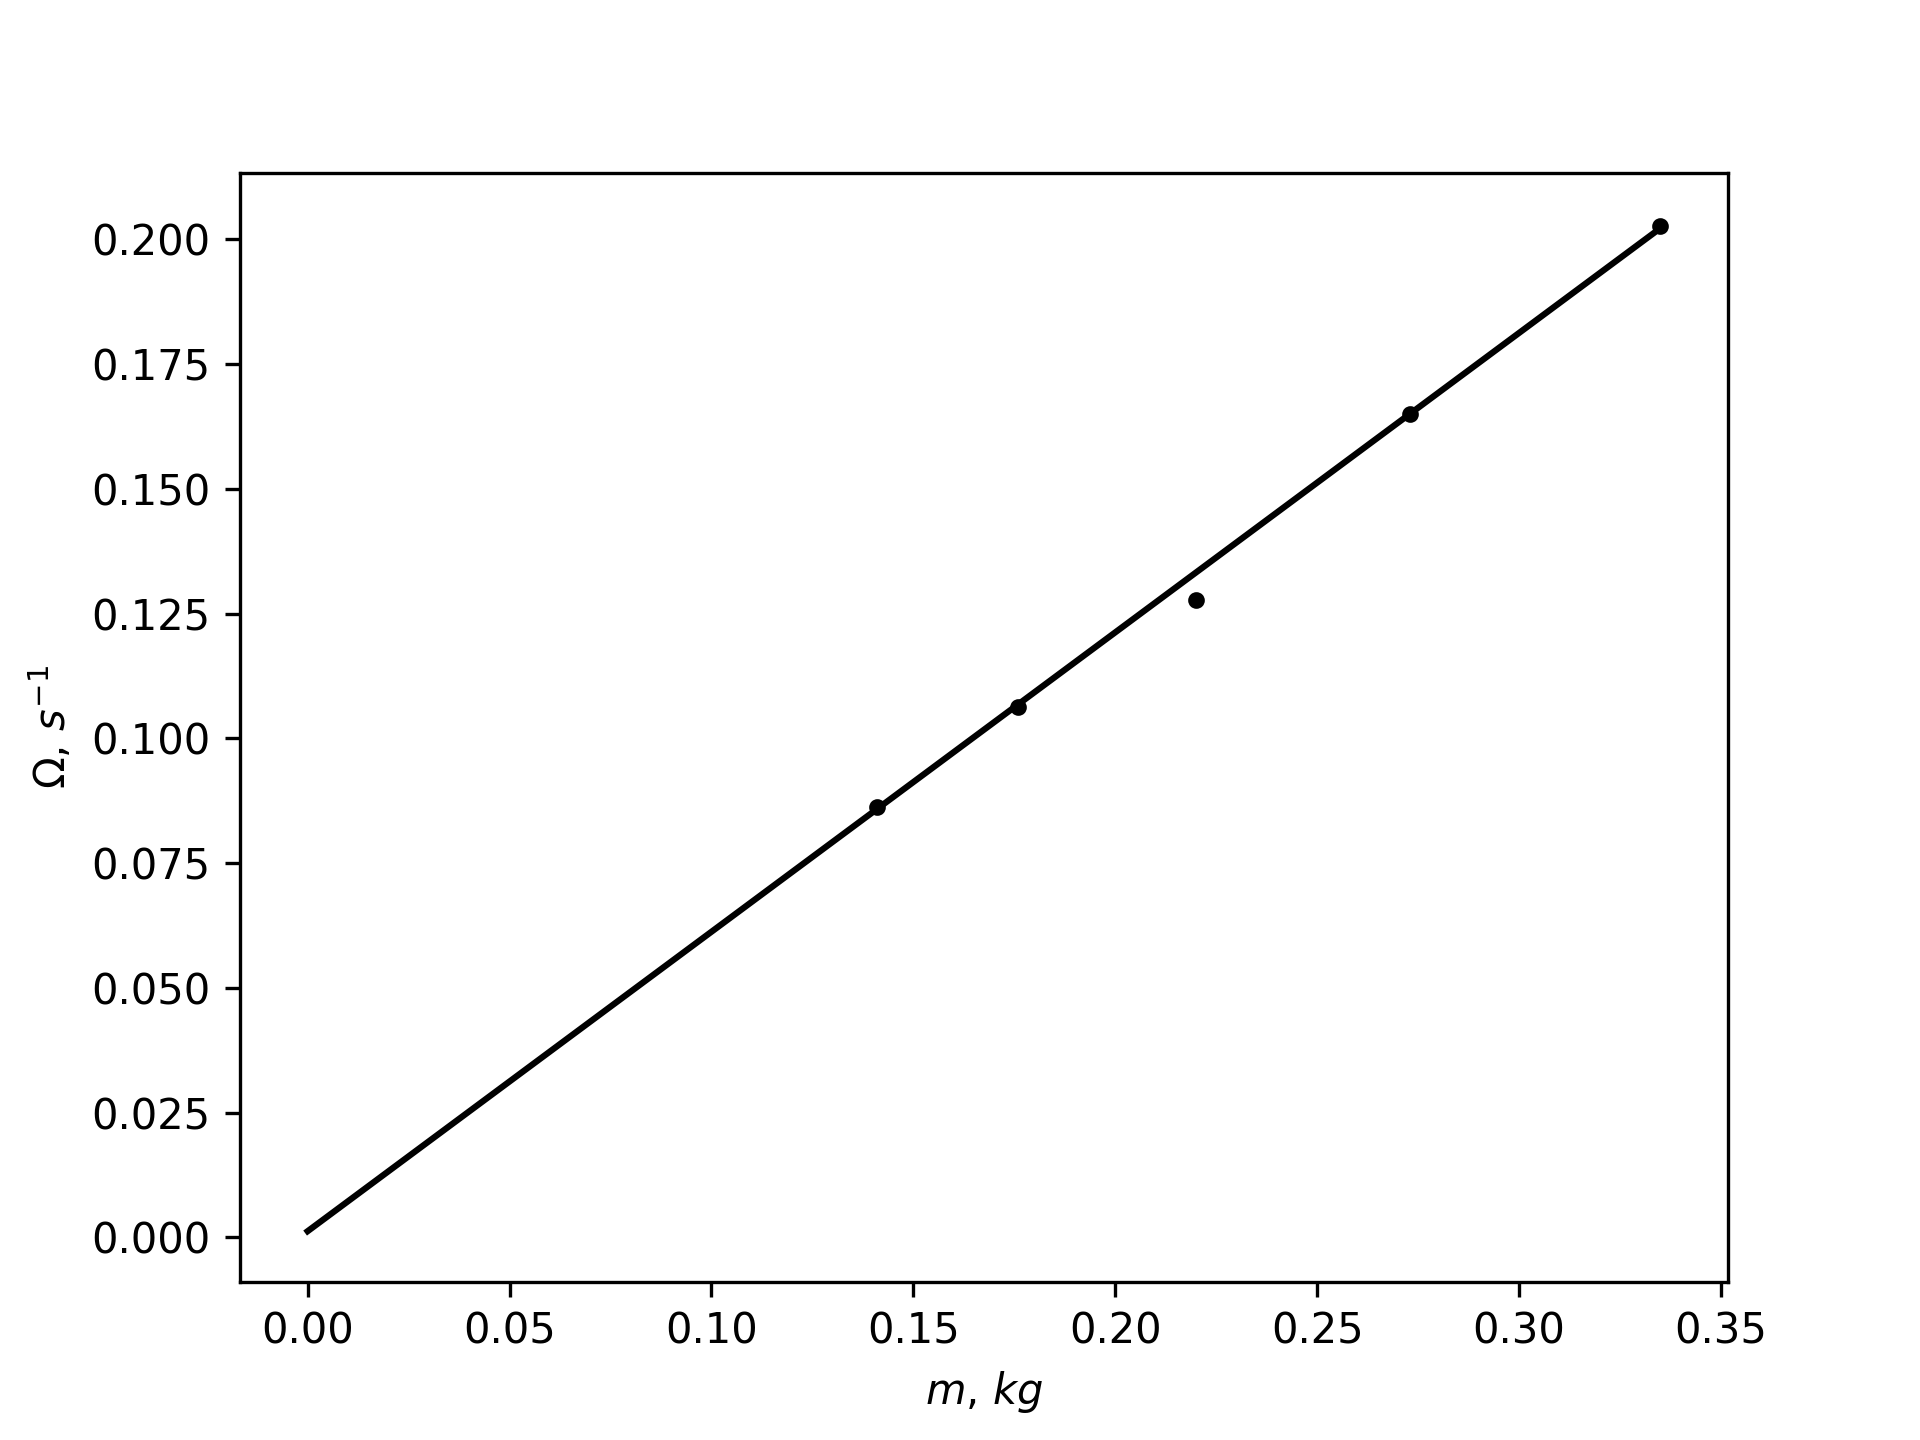
\includegraphics[scale=0.75]{laba8_1.png}
\caption{График зависимости $\Omega(m)$}
\end{figure}

\[k=(599,9\pm2.6)\cdot10^{-3}\ kg^{-1}s^{-1}\]

С другой стороны, коэффициент $k$ может быть выражен следующим образом:
\[\Omega=\frac{mgl}{I_g\omega}=km\]
\[k=\frac{gl}{I_g\omega}\]

Момент инерции $I_g$ определим с помощью крутильного маятник, измерив период колебаний гироскопа и сплошного цилиндра.

\begin{table}[!h]
\centering
\begin{tabular}{| c | c |}
\hline
Масса цилиндра, $m_c$, $g$ & $1616.8\pm0.1$ \\
Диаметра цилиндра $d_c$, $mm$ & $78\pm0.1$ \\
Период колебаний цилиндра $T_c$, $s$ & $4.16\pm0.01$ \\
Период колебаний гироскопа $T_g$, $s$ & $3.32\pm0.01$ \\
\hline
\end{tabular}
\label{table3}
\caption{Вычисление момента инерции гироскопа}
\end{table}

В таком случае момент инерции $I_g$ может быть рассчитан следующим образом:
\[I_c=\frac{1}{2}m_c\frac{d_c^2}{4}=\frac{1}{8}m_cd_c^2\]
\[I_g=I_c\frac{T_g^2}{T_c^2}=\frac{1}{8}m_cd_c^2\frac{T_g^2}{T_c^2}\]
\[\sigma_{I_g}=I_g\sqrt{\left(\frac{\sigma_{m_c}}{m_c}\right)^{2}+\left(2\frac{\sigma_{d_c}}{d_c}\right)^{2}+\left(2\frac{\sigma_{T_c}}{T_c}\right)^{2}+\left(2\frac{\sigma_{T_g}}{T_g}\right)^{2}}\]
\[I_g=(786.1\pm6.4)\cdot10^{-6}\ kg\cdot m^{-2}\]

Далее может быть найдена частота вращения гироскопа:
\[\nu=\frac{gl}{2\pi I_gk},\ \sigma_\nu=\nu\sqrt{\left(\frac{\sigma_{I_g}}{I_g}\right)^{2}+\left(\frac{\sigma_{k}}{k}\right)^{2}}\]
\[\nu=400.8\pm3.7\ Hz\]

Измерения проведенные с помощью генератора и осциллографа возвращают значение:
\[\nu_0=390.9\ Hz\]

\end{document}